\documentclass[border=6pt]{standalone}
\usepackage[T1]{fontenc}
\usepackage{times}
\usepackage{amsmath,amssymb}
\usepackage{xcolor}
\usepackage{tikz}
\usetikzlibrary{positioning,arrows.meta,shapes.geometric,fit,calc,backgrounds}
\definecolor{wm}{HTML}{2E6DB4}
\definecolor{jp}{HTML}{E07B1A}
\definecolor{ph}{HTML}{2E8B57}
\definecolor{gr}{HTML}{6B6B6B}
\begin{document}
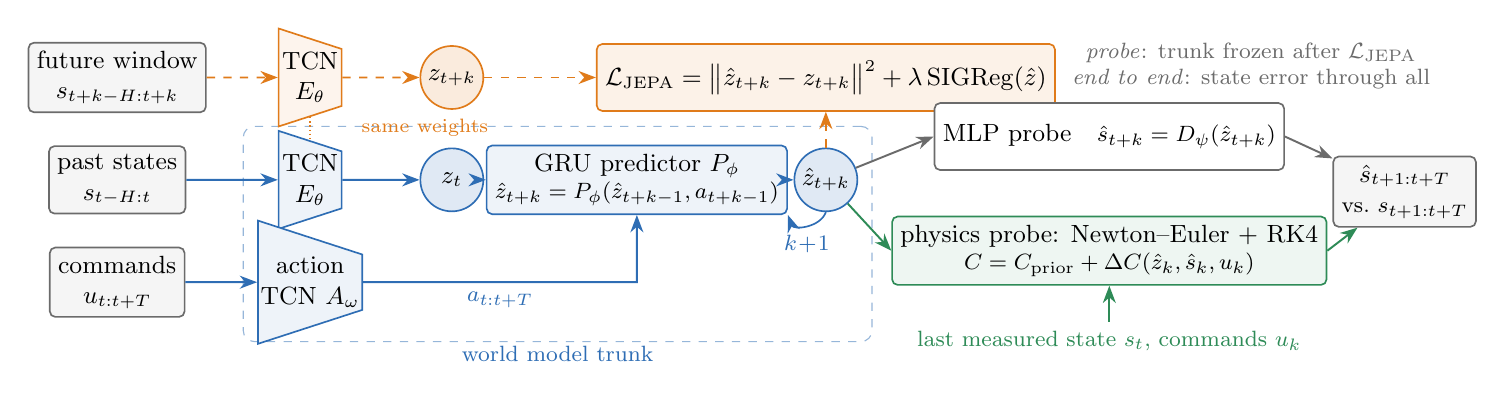
\begin{tikzpicture}[font=\small, >={Stealth[length=2.2mm]},
  box/.style={draw, rounded corners=2pt, align=center, minimum height=8.5mm, inner sep=3pt, line width=0.6pt},
  enc/.style={trapezium, trapezium angle=72, shape border rotate=270, draw, align=center, minimum height=8mm, inner sep=1pt, line width=0.6pt},
  lat/.style={circle, draw, inner sep=1pt, minimum size=8mm, line width=0.6pt},
  data/.style={box, fill=gray!8, draw=gr}]
  % ---- online branch (world model trunk)
  \node[data] (past) at (0,0) {past states\\$s_{t-H:t}$};
  \node[enc, draw=wm, fill=wm!8] (E) at (2.45,0) {TCN\\$E_\theta$};
  \node[lat, draw=wm, fill=wm!15] (z0) at (4.25,0) {$z_t$};
  \node[data] (cmd) at (0,-1.3) {commands\\$u_{t:t+T}$};
  \node[enc, draw=wm, fill=wm!8] (A) at (2.45,-1.3) {action\\TCN $A_\omega$};
  \node[box, draw=wm, fill=wm!8, minimum width=27mm] (P) at (6.6,0) {GRU predictor $P_\phi$\\[-1pt]{\footnotesize $\hat z_{t+k}=P_\phi(\hat z_{t+k-1}, a_{t+k-1})$}};
  \node[lat, draw=wm, fill=wm!15] (zh) at (9.0,0) {$\hat z_{t+k}$};
  \draw[->, wm, line width=0.7pt] (past) -- (E);
  \draw[->, wm, line width=0.7pt] (E) -- (z0);
  \draw[->, wm, line width=0.7pt] (z0) -- (P);
  \draw[->, wm, line width=0.7pt] (cmd) -- (A);
  \draw[->, wm, line width=0.7pt] (A) -- node[below, font=\footnotesize]{$a_{t:t+T}$} (A -| P) -- (P);
  \draw[->, wm, line width=0.7pt] (P) -- (zh);
  \draw[->, wm, line width=0.6pt] (zh.south) to[out=-110,in=-70, looseness=1.1] node[below, font=\footnotesize]{$k\!+\!1$} (P.south east);
  % ---- target branch (JEPA)
  \node[data] (fut) at (0,1.3) {future window\\$s_{t+k-H:t+k}$};
  \node[enc, draw=jp, fill=jp!8] (Et) at (2.45,1.3) {TCN\\$E_\theta$};
  \node[lat, draw=jp, fill=jp!15] (zt) at (4.25,1.3) {$z_{t+k}$};
  \node[box, draw=jp, fill=jp!10] (LJ) at (9.0,1.3) {$\mathcal L_{\mathrm{JEPA}}=\big\|\hat z_{t+k}-z_{t+k}\big\|^2+\lambda\,\mathrm{SIGReg}(\hat z)$};
  \draw[->, jp, dashed, line width=0.7pt] (fut) -- (Et);
  \draw[->, jp, dashed, line width=0.7pt] (Et) -- (zt);
  \draw[->, jp, dashed, line width=0.7pt] (zt) -- (LJ);
  \draw[->, jp, dashed, line width=0.7pt] (zh) -- (LJ);
  \draw[jp, densely dotted, line width=0.5pt] (Et.south) -- (E.north);
  \node[font=\scriptsize, jp, anchor=west] at (2.98,0.66) {same weights};
  % ---- readouts
  \node[box, draw=gr, fill=white, minimum width=30mm] (mlp) at (12.6,0.55) {MLP probe\quad{\footnotesize $\hat s_{t+k}=D_\psi(\hat z_{t+k})$}};
  \node[box, draw=ph, fill=ph!8, minimum width=30mm] (phy) at (12.6,-0.9) {physics probe: Newton--Euler + RK4\\[-1pt]
     {\footnotesize $C=C_{\mathrm{prior}}+\Delta C(\hat z_k,\hat s_k,u_k)$}};
  \draw[->, line width=0.7pt, gr] (zh) -- (mlp.west);
  \draw[->, line width=0.7pt, ph] (zh) -- (phy.west);
  \node[font=\footnotesize, ph, align=center] (s0) at (12.6,-2.05) {last measured state $s_t$, commands $u_k$};
  \draw[->, line width=0.6pt, ph] (s0) -- (phy.south);
  \node[box, draw=gr, fill=gray!8] (sh) at (16.35,-0.15) {$\hat s_{t+1:t+T}$\\{\footnotesize vs.\ $s_{t+1:t+T}$}};
  \draw[->, line width=0.7pt, gr] (mlp.east) -- (sh);
  \draw[->, line width=0.7pt, ph] (phy.east) -- (sh);
  \node[font=\footnotesize, align=center, gr] at (14.4,1.45) {\emph{probe}: trunk frozen after $\mathcal L_{\mathrm{JEPA}}$\\\emph{end to end}: state error through all};
  \begin{scope}[on background layer]
    \node[draw=wm!50, dashed, rounded corners=4pt, fit=(E)(A)(P)(zh)(z0), inner sep=5pt, label={[font=\footnotesize, wm, yshift=2pt]below:{world model trunk}}] {};
  \end{scope}
\end{tikzpicture}
\end{document}
